\Problem
{گام پنجم}
{
با استفاده از دستور \lr{huffmandict} که یک الفبا و یک توزیع احتمال می‌گیرد، دیکشنری هافمن را می‌سازیم.

برای تولید الفبا و کوانتیزه کردن ورودی از دستور \lr{quantiz} 
استفاده کردیم.

پس از تولید الفبا، با استفاده از دستور \lr{huffmanenco} 
رشته کد شده را تولید و درون فایل صوتی جدید ذخیره می‌کنیم.

\begin{figure}[H]
    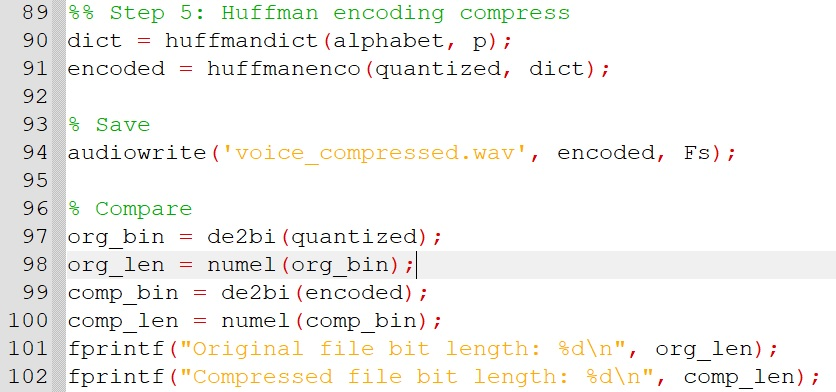
\includegraphics[width=15cm]{Images/step_5_code.jpg}
    \centering
    \caption{کد مربوط به گام پنجم}
\end{figure}

سپس طول بیتی که برای حالت اولیه و حالت فشرده سازی شده لازم است را محاسبه می‌کنیم. خروجی به صورت زیر است:

\begin{latin}
\newline
Original file bit length: 349848
\newline
Compressed file bit length: 181565
\newline
\end{latin}
}

همانطور که مشاهده می‌شود تعداد بیت مورد نیاز پس از فشرده سازی کمتر شده است. اما پس از ذخیره سازی متوجه می‌شویم حجم فایل بیشتر شده است. دلیل آن این است که فایل اولیه خود مکانیزمی برای فشرده سازی خود داشته است که ما با باز کردن آن و تبدیل آن به بیت آن فشرده سازی اولیه را از بین برده ایم.

زمان لازم برای انتقال با لینک توصیف شده به صورت زیر به دست می‌آید:

\begin{equation*}
    Original = 349848 / (64 * 1000) = 5.46 [s]
\end{equation*}

\begin{equation*}
    Compressed = 181565 / (64 * 1000) = 2.83 [s]
\end{equation*}

که تقریبا این زمان نصف شده است.